\subsection{OAuth e OAuth 2.0}

O protocolo OAuth foi especificado na RFC 5849, fornecendo um método para clientes acessarem 
recursos de um servidor em nome de um proprietário de recurso e também um processo para que os 
usuários finais autorizem o acesso de terceiros aos seus recursos de servidor sem compartilhar suas
credenciais \cite{RFC5849}. Este método de autenticação funciona seguindo as seguintes etapas:

\begin{itemize}
\item O usuário solicita o serviço de um sistema, chamado de cliente;
\item O cliente, tendo previamente configurado acesso ao servidor de recursos, possuindo um 
identificador e um segredo compartilhado, envia uma solicitação a este servidor para receber um 
\emph{token} de solicitação;
\item O servidor valida a solicitação, enviando o \emph{token} de solicitação não-autorizado no 
corpo da resposta HTTP;
\item O cliente redireciona o agente do usuário para o servidor, que solicita o \emph{login} do 
usuário e depois a autorização para o cliente acessar o recurso;
\item O cliente recebe um \emph{token} de solicitação, que utiliza em uma nova solicitação por 
\emph{token} de acesso. Estas requisições são realizadas por meio de um canal TLS;
\item O servidor valida o \emph{token} de solicitação e envia o \emph{token} de acesso ao cliente e 
opcionalmente um \emph{token} de atualização;
\item O cliente utiliza o \emph{token} de acesso para solicitar os recursos do servidor.
\end{itemize}

Na RFC 6749 foi proposto o protocolo OAuth 2.0, tornando obsoleta sua versão anterior. Esta versão possui 
poucas semelhanças com a versão anterior, utilizando os mesmos princípios mas com fluxo diferente e 
abrangendo mais casos de uso, além de estabelecer o uso do protocolo HTTPS, possuindo todas as mensagens 
criptografadas. Por este motivo os dois protocolos não são compatíveis, coexistindo e podendo ambos serem 
suportados pelos sistemas \cite{RFC6749}. Diferente da versão 1.0, que depende de assinaturas 
criptografadas para cada requisição, a versão 2.0 utiliza \emph{tokens} portadores (\emph{bearer tokens}) 
que são protegidos devido ao uso do TLS \cite{SIRIWARDENA2014}. Seu funcionamento é dado pelas seguintes 
etapas (Figura \ref{fig:OAuth2}):

\begin{itemize}
\item O cliente solicita permissão de acesso ao usuário;
\item O cliente recebe a permissão e solicita um \emph{token} de acesso ao servidor de autenticação;
\item O servidor de autenticação autentica o cliente e valida suas permissões, enviando a ele o 
\emph{token} de acesso e opcionalmente um \emph{token} de atualização;
\item O cliente solicita o recurso protegido ao servidor de recursos, que valida o \emph{token} de 
acesso e atende a solicitação.
\end{itemize}

\begin{figure}[ht]
    \centering
    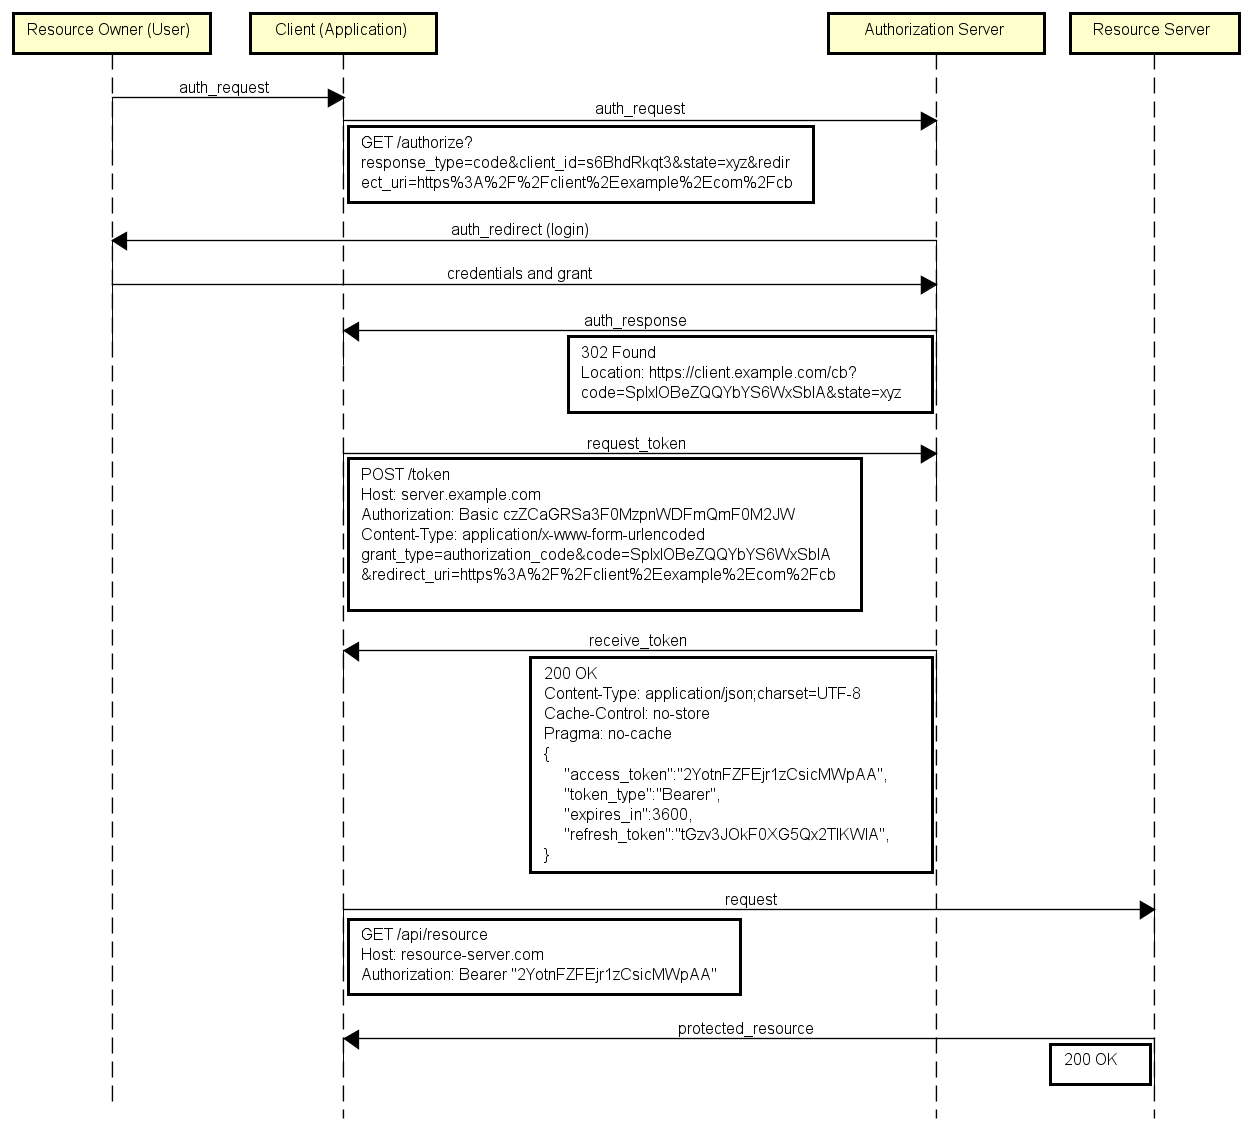
\includegraphics[width=1\textwidth]{OAuth 2.0.png}
    \caption{Exemplo de autenticação utilizando OAuth 2.0}
    \label{fig:OAuth2}
\end{figure}